\documentclass[11pt]{article}
\usepackage{microtype}
\usepackage{graphicx}
\usepackage{wrapfig}
\usepackage{url}
\usepackage{wrapfig}
\usepackage{color}
\usepackage{marvosym}
\usepackage{enumerate}
\usepackage{subfigure}
\usepackage{tikz}
\usepackage[fleqn]{amsmath}
\DeclareMathOperator*{\argmax}{arg\,max}
\DeclareMathOperator*{\argmin}{arg\,min}
\usepackage{amssymb}
\usepackage{hyperref}
\usepackage[many]{tcolorbox}
\usepackage{lipsum}
\usepackage{float}
\usepackage{trimclip}
\usepackage{listings}
\usepackage{environ}% http://ctan.org/pkg/environ
\usepackage{wasysym}
\usepackage{array}
\usepackage{cancel}

\newcommand{\Angie}[1]{\textcolor{blue}{Angie - #1}}
\newcommand{\Xuan}[1]{\textcolor{green}{Xuan - #1}}


\oddsidemargin 0mm
\evensidemargin 5mm
\topmargin -20mm
\textheight 240mm
\textwidth 160mm

\newcommand{\vwi}{{\bf w}_i}
\newcommand{\vw}{{\bf w}}
\newcommand{\vx}{{\bf x}}
\newcommand{\vy}{{\bf y}}
\newcommand{\vxi}{{\bf x}_i}
\newcommand{\yi}{y_i}
\newcommand{\vxj}{{\bf x}_j}
\newcommand{\vxn}{{\bf x}_n}
\newcommand{\yj}{y_j}
\newcommand{\ai}{\alpha_i}
\newcommand{\aj}{\alpha_j}
\newcommand{\X}{{\bf X}}
\newcommand{\Y}{{\bf Y}}
\newcommand{\vz}{{\bf z}}
\newcommand{\msigma}{{\bf \Sigma}}
\newcommand{\vmu}{{\bf \mu}}
\newcommand{\vmuk}{{\bf \mu}_k}
\newcommand{\msigmak}{{\bf \Sigma}_k}
\newcommand{\vmuj}{{\bf \mu}_j}
\newcommand{\msigmaj}{{\bf \Sigma}_j}
\newcommand{\pij}{\pi_j}
\newcommand{\pik}{\pi_k}
\newcommand{\D}{\mathcal{D}}
\newcommand{\el}{\mathcal{L}}
\newcommand{\N}{\mathcal{N}}
\newcommand{\vxij}{{\bf x}_{ij}}
\newcommand{\vt}{{\bf t}}
\newcommand{\yh}{\hat{y}}
\newcommand{\code}[1]{{\footnotesize \tt #1}}
\newcommand{\alphai}{\alpha_i}
\newcommand{\defeq}{\overset{\text{def}}{=}}
\renewcommand{\vec}[1]{\mathbf{#1}}



\bgroup
\def\arraystretch{1.5}
\newcolumntype{x}[1]{>{\centering\arraybackslash\hspace{0pt}}p{#1}}
\newcolumntype{z}[1]{>{\centering\arraybackslash}m{#1}}

%Arguments are 1 - height, 2 - box title
\newtcolorbox{textanswerbox}[2]{%
 width=\textwidth,colback=white,colframe=blue!30!black,floatplacement=H,height=#1,title=#2,clip lower=true,before upper={\parindent0em}}

 \newtcolorbox{eqanswerbox}[1]{%
 width=#1,colback=white,colframe=black,floatplacement=H,height=3em,sharp corners=all,clip lower=true,before upper={\parindent0em}}

 %Arguments are 1 - height, 2 - box title
 \NewEnviron{answertext}[2]{
        \noindent
        \marginbox*{0pt 10pt}{
        \clipbox{0pt 0pt 0pt 0pt}{
        \begin{textanswerbox}{#1}{#2}
        \BODY
        \end{textanswerbox}
        }
        }
}

%Arguments are 1 - height, 2 - box title, 3 - column definition
 \NewEnviron{answertable}[3]{
        \noindent
        \marginbox*{0pt 10pt}{
        \clipbox{0pt 0pt 0pt 0pt}{
        \begin{textanswerbox}{#1}{#2}
                \vspace{-0.5cm}
                        \begin{table}[H]
                        \centering
                        \begin{tabular}{#3}
                                \BODY
                        \end{tabular}
                        \end{table}
        \end{textanswerbox}
        }
        }
}

 %Arguments are 1 - height, 2 - box title, 3 - title, 4- equation label, 5 - equation box width
 \NewEnviron{answerequation}[5]{
        \noindent
        \marginbox*{0pt 10pt}{
        \clipbox{0pt 0pt 0pt 0pt}{
        \begin{textanswerbox}{#1}{#2}
                \vspace{-0.5cm}
                        \begin{table}[H]
                        \centering
                \renewcommand{\arraystretch}{0.5}% Tighter

                        \begin{tabular}{#3}
                                #4 =	&
                        \clipbox{0pt 0pt 0pt 0pt}{

                        \begin{eqanswerbox}{#5}
                                $\BODY$
                        \end{eqanswerbox}
                        } \\
                        \end{tabular}
                        \end{table}

        \end{textanswerbox}
        }
        }
}

 %Arguments are 1 - height, 2 - box title
 \NewEnviron{answerderivation}[2]{
        \noindent
        \marginbox*{0pt 10pt}{
        \clipbox{0pt 0pt 0pt 0pt}{
        \begin{textanswerbox}{#1}{#2}
        \BODY
        \end{textanswerbox}
        }
        }
}

\newcommand{\Checked}{{\LARGE \XBox}}%
\newcommand{\Unchecked}{{\LARGE \Square}}%
\newcommand{\TextRequired}{{\textbf{Place Answer Here}}}%
\newcommand{\EquationRequired}{\textbf{Type Equation Here}}%


\newcommand{\answertextheight}{5cm}
\newcommand{\answertableheight}{4cm}
\newcommand{\answerequationheight}{2.5cm}
\newcommand{\answerderivationheight}{14cm}

\newcounter{QuestionCounter}
\newcounter{SubQuestionCounter}[QuestionCounter]
\setcounter{SubQuestionCounter}{1}

\newcommand{\subquestiontitle}{Question \theQuestionCounter.\theSubQuestionCounter~}
\newcommand{\newquestion}{\stepcounter{QuestionCounter}\setcounter{SubQuestionCounter}{1}\newpage}
\newcommand{\newsubquestion}{\stepcounter{SubQuestionCounter}}


\lstset{language=[LaTeX]TeX,basicstyle=\ttfamily\bf}

\pagestyle{myheadings}
\markboth{Homework 5}{Fall 2022 CS 475/675 Machine Learning: Homework 5}

\title{CS 475/675 Machine Learning: Homework 5\\
Analytical Questions\\
\Large{12 Points Total \hspace{1cm} Version 1.0}
\author{PARTNER1\_NAME, PARTER2\_NAME, $\ldots$ \\
PARTNER1\_JHED, PARTNER2\_JHED, $\ldots$}}
\date{}

\begin{document}
\maketitle
\thispagestyle{headings}


\section*{Instructions }
We have provided this \LaTeX{} document for completing the analytical portion of the assignment. We give you one or more boxes to answer each question.  The question to answer for each box will be noted in the title of the box.\\

{\bf Other than your name, do not type anything outside the boxes. Leave the rest of the document unchanged.}\\


\textbf{Do not change any formatting in this document, or we may be unable to
  grade your work. This includes, but is not limited to, the height of
  textboxes, font sizes, and the spacing of text and tables.  Additionally, do
  not add text outside of the answer boxes. Entering your answers are the only
  changes allowed.}\\


\textbf{We strongly recommend you review your answers in the generated PDF to
  ensure they appear correct. We will grade what appears in the answer boxes in
  the submitted PDF, NOT the original latex file.}

\pagebreak

\newquestion
\section*{\arabic{QuestionCounter}) 
Graphical Models (3 points)} 

Consider the Directed Acyclic Graph (DAG) in the following figure. $X_1, X_2, ..., X_{10}$ are random variables.

\begin{figure}[h]
\begin{center}
\scalebox{0.9}{
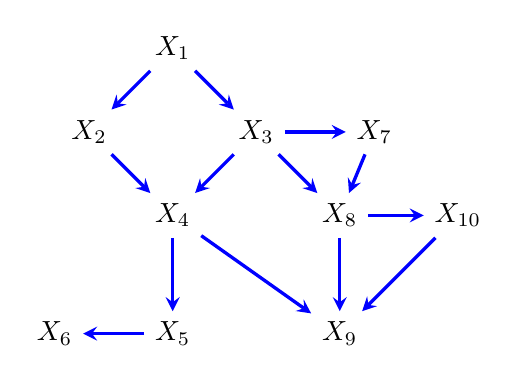
\begin{tikzpicture}[>=stealth, node distance=1.5cm]
    \tikzstyle{format} = [draw, thick, circle, minimum size=1.0mm, inner sep=0pt]
	\tikzstyle{square} = [draw, thick, minimum size=1.0mm, inner sep=3pt]
	\begin{scope}
		\path[->, very thick]
			node[] (x1) {$X_1$}
			node[below left of=x1] (x2) {$X_2$}
			node[below right of=x1] (x3) {$X_3$}		
			node[right of=x3] (x7) {$X_7$}
			node[below right of=x3] (x8) {$X_8$}
			node[below left of=x3] (x4) {$X_4$}
			node[right of=x8] (x10) {$X_{10}$}
			node[below of=x8] (x9) {$X_9$}
			node[below of=x4] (x5) {$X_5$}
			node[left of=x5] (x6) {$X_6$}
			(x1) edge[blue] (x2)
			(x1) edge[blue] (x3)
			(x2) edge[blue] (x4)
			(x3) edge[blue] (x7)
			(x3) edge[blue] (x4)
			(x3) edge[blue] (x8)
			(x4) edge[blue] (x5)
			(x4) edge[blue] (x9)
			(x5) edge[blue] (x6)
			(x7) edge[blue] (x8)
			(x8) edge[blue] (x9)
			(x8) edge[blue] (x10)
			(x10) edge[blue] (x9)
			;
	\end{scope}
\end{tikzpicture}
}
\end{center}
\label{fig:prob1}
\end{figure}



% \item (3 point) There are 9 independencies that can be read off the given Directed Acyclic Graph (DAG) using the local Markov property. List all of them, one for each $X_i$, where $i \in \{2, 3, 4, 5, 6, 7, 8, 9, 10\}$. \\
% % add symbol
% % make hint to the question
% % explain 
% \textit{Hint: The local Markov propery states that any random variable $X_i$ is conditionally independent of all other random variables that are not its descendants in the DAG, given $X_i$'s parents.}\\
% \begin{answertext}{12cm}{}
% According to he local Markov property any node $\{X_i \perp_d \textrm{non\_descendents}(X_i, G) \mid parents(X_i, G)\}$. Here $G$ refers to the given DAG. Following are the independencies characterized by the give DAG $G$. 
% \begin{itemize}
%     \item $X_2 \perp_d \{X_3, X_7, X_8, X_{10}\} \mid X_1$ \\
%     \item $X_3 \perp_d X_2 \mid X_1$ \\
%     \item $X_4 \perp_d \{X_1, X_7, X_8, X_{10}\} \mid \{X_2, X_3\}$ \\
%     \item $X_5 \perp_d \{X_1, X_2, X_3, X_7, X_8, X_9, X_{10}\} \mid X_4$ \\
%     \item $X_6 \perp_d \{X_1, X_2, X_3, X_4, X_7, X_8, X_9, X_{10}\} \mid X_5$ \\
%     \item $X_7 \perp_d \{X_1, X_2, X_4, X_5, X_6\} \mid X_3$ \\
%     \item $X_8 \perp_d \{X_1, X_2, X_4, X_5, X_6\} \mid \{X_3, X_7\}$ \\
%     \item $X_9 \perp_d \{X_1, X_2, X_3, X_5, X_6, X_7\} \mid \{X_4, X_8, X_{10}\}$ \\
%     \item $X_{10} \perp_d \{X_1, X_2, X_3, X_4, X_5, X_6, X_7\} \mid X_8$.
% \end{itemize}
% \end{answertext}
% \newpage
Answer the following three questions. The symbol $\perp_d$ means independent. If your answer is No, explain why. 
\begin{enumerate}[(a)]
    \item Is $X_2 \perp_d X_9 | X_4$?
    \item Is $X_7 \perp_d X_5 | \{X_3, X_8 \}$?
    \item Is $ \{X_2, X_4\} \perp_d X_7 | \{X_6, X_9, X_{10} \}$?
\end{enumerate}

\begin{answertext}{13cm}{}
% \begin{enumerate}[(a)]
%     \item Is $X_2 \perp_d X_9 | X_4$? No. There is an active path through $X_1$.
%     \item Is $X_7 \perp_d X_5 | {X_3, X_8}$? Yes.
%     \item Is $ \{X_2, X_4\} \perp_d X_7 | \{X_6, X_9, X_{10} \}$? No. There is an active path through active collider $X_9$ or through $X_3$.
% \end{enumerate}
\end{answertext}


\newquestion
\section*{\arabic{QuestionCounter}) 
Expectation Maximization (9 points)} 

Consider two biased coins $A$ and $B$ with success probability (probability of obtaining head) $p_A$ and $p_B$ respectively. We have access to a sequence of 10 independent coin tosses ``$THTTTTTHHT$",\footnote{$H$ represents a heads and $T$ represents a tails.} however we do not know in advance which coin was used in each toss.

We would illustrate how the EM algorithm can be used to learn the parameters $p_A$ and $p_B$.\footnote{Note, this is a toy illustration in practice you would need much more than 10 coin tosses to get accurate estimates of $p_A$ and $p_B$.} Let's assume initial estimates of $p_A$ and $p_B$ to be $\hat{p}_A$ and $\hat{p}_B$ respectively.

\begin{enumerate}[(1)]
\item (3 points) Since we do not know which coin was used for which toss, we would model this as a hidden variable $Z$. Let $Z = 1$ indicate coin A was chosen and $Z = 0$ indicate that coin B was chosen. We can then express the probability of observing an heads on any toss as 
\begin{equation}
    P(X_i = H) = P(X_i = H \mid Z = 1)P(Z = 1) + P(X_i = H \mid Z = 0)P(Z = 0),
    \label{eq: forward model}
\end{equation}
where $i$ refers the to index of the toss, however since each coin toss is i.i.d, the distribution for all $X_i$ would be identical. You are given prior information that $P(Z = 0) = P(Z = 1) = 0.5$. Using \eqref{eq: forward model}, compute the posterior $P(Z = 1 \mid X_i = H)$ in terms of $\hat{p}_A$ and $\hat{p}_B$.\\
\textit{Hint: Use the Bayes' Theorem. $p_A = P(X_i = H \mid Z = 1)$ and $p_B = P(X_i = H \mid Z = 0)$. }

\begin{answertext}{10cm}{}
% \begin{equation}
% \begin{aligned}
%      P(Z = 1 \mid X_i = H) &= \frac{P(X_i = H \mid Z = 1)P(Z = 1) }{P(X_i = H \mid Z = 1)P(Z = 1) + P(X_i = H \mid Z = 0)P(Z = 0)}\nonumber
%     \\
%     &= \frac{\hat{p}_A}{\hat{p}_A + \hat{p}_B}
% \end{aligned}
% \end{equation}
\end{answertext}

\item (6 points) The EM algorithm proceeds by starting with initial estimates $\hat{p}_A$ and $\hat{p}_B$ and computes the expected complete data log likelihood (E-step). It then updates its estimates by maximizing this expected complete data log-likelihood by keeping the posteriors fixed (M-step). You will compute some key steps for both steps.

\begin{enumerate}[(2.1)]
\item (4 points) (E-Step) Start with initial estimates $\hat{p}_A = 0.6$ and $\hat{p}_B = 0.8$. Using these values compute the value of every posterior $\tau_{\alpha, \beta} = P(Z = \alpha \mid X_i = \beta)$, where $\alpha \in \{0, 1\}$ and $\beta \in \{H, T\}$. 

With these computed $\tau_{\alpha, \beta}$ values, we would \textit{update our estimates} for $p_A$ and $p_B$. To do this, first express the expected complete data log-likelihood for the sequence ``$THTTTTTHHT$" in terms of $\tau_{\alpha, \beta}$, and \textit{variables} $p_A$ and $p_B$.  Then calculate the expected complete data log-likelihood $L$, where you can substitute the values computed for $\tau_{\alpha, \beta}$.

\textit{Hint: Recall $P(Z = 0) = P(Z = 1) = 0.5$. The complete data log-likelihood is defined as follows,
\[L = \sum_{i=1}^N\sum_{\alpha=0}^1\tau_{\alpha, x_i}\log p(X_i = x_i, Z = \alpha).\]
Here $X_i$ is the random variable indicating the outcome of the $i^{\textrm{th}}$ toss. For example $X_1 = x_1 = T$, $X_2 = x_2 = H$ and so on. }

\begin{answertext}{17cm}{}
% \begin{equation}
%     \begin{aligned}
%     \tau_{0, H} &= \frac{0.8}{0.6 + 0.8} &= 0.57\nonumber \\
%     \tau_{0, T} &= \frac{0.2}{0.4 + 0.2} &= 0.33 \\
%     \tau_{1, H} &= \frac{0.6}{0.6 + 0.8} &= 0.43 \\
%     \tau_{1, T} &= \frac{0.4}{0.4 + 0.2} &= 0.67 \\
%     \end{aligned}
% \end{equation}

% \begin{equation}
% \begin{aligned}
%      L &=  \sum_{i=1}^N\sum_{\alpha=0}^1\tau_{\alpha, x_i}\log p(X_i = x_i, Z = \alpha) \nonumber\\
%      &= \frac{1}{2} \left[7\left(\tau_{1, T}\log (1 - p_A) + \tau_{0, T}\log (1 - p_B)\right) + 3\left(\tau_{1, H}\log p_A + \tau_{0, H}\log p_B \right) \right] \\ 
%      &= \frac{1}{2}\left[7\left(0.67\log (1 - p_A) + 0.33\log (1 - p_B)\right) + 3\left(0.43\log p_A + 0.57\log p_B \right) \right] \\
%      &= \frac{1}{2}\left[4.69(\log (1 - p_A)) + 2.31(\log (1 - p_B)) + 1.29(\log p_A) + 1.71\log p_B) \right] \\
%      &= 2.345(\log (1 - p_A)) + 1.155(\log (1 - p_B)) + 0.645(\log p_A) + 0.855\log p_B))
% \end{aligned}
% \end{equation}
\end{answertext}

\item (2 points) (M-Step) We would now update our estimates for $p_A$ and $p_B$ by maximizing $L$ (the expected complete data likelihood). Calculate the new values of $p_A$ and $p_B$. 
\textit{Hint: You would do this by considering the partial derivative of $L$ w.r.t $p_A$ and $p_B$ respectively and equating it to $0$ (to find the local maximum).} Please only answer the values of $p_A$ and $p_B$, partial derivatives are optional.


\begin{answertext}{10cm}{}
% Computing the partial derivatives and equating to we get the following solutions,
% \begin{equation}
% \begin{aligned}
%      p_A &= 0.2157 \nonumber\\
%      p_B &= 0.425
% \end{aligned}
% \end{equation}
\end{answertext}
% Thus, we refine our original estimates of $\hat{p}_A$ and $\hat{p_B}$ to the new values you obtained in the above problem by setting the partial derivatives to $0$, recompute the $\tau_{\alpha, \beta}$ based on these updated estimates and alternate until convergence.

\end{enumerate}



\end{enumerate}


\end{document}